\documentclass[answers]{exam}
\input{global}
\input{problem-sets}


\setrandomizerseed{2}
\bracketedpoints


\firstpageheader{{Name:\enspace\makebox[5cm]{\hrulefill}}\\Physics}{}{Test on Unit 1: Constant Velocity\\}
\runningheader{Physics}{}{Test on Unit 1: Constant Velocity}


\begin{document}

\begin{questions}

\question 
The figure below shows the one-dimensional motion of a particle. 

\begin{center}
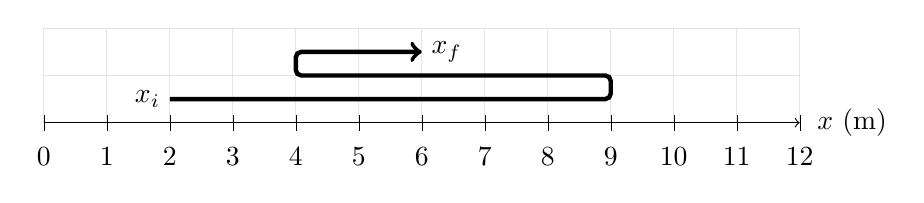
\begin{tikzpicture}[y=3mm,x=8mm]
    \draw[black!10,xstep=1,ystep=2] (0,0) grid (12,4);
    \foreach \x in {0,1,...,12} {
        \draw[ultra thin] (\x,-1mm) -- (\x,1mm) node[below=3mm] {$\x$};
    }
    \draw[->] (0,0) -- (12,0) node[right=1mm] {$x$ (m)};
    \draw[ultra thick,->,rounded corners=0.7mm] (2,1)
        -- (9,1) 
        -- (9,2) 
        -- (4,2) 
        -- (4,3) 
        -- (6,3);
    \node[left] at (2,1) {$x_i$};
    \node[right] at (6,3) {$x_f$};
\end{tikzpicture}
\end{center}

Calculate the total distance traveled.

\begin{randomizechoices}
    \correctchoice \SI{14}{m}
    \choice \SI{6}{m}
    \choice \SI{16}{m}
    \choice \SI{4}{m}
\end{randomizechoices}

\question
A cyclist travels 45 meters in 9 seconds. What is her average speed?

\begin{randomizechoices}
    \correctchoice \SI{5}{m/s}
    \choice \SI{0.2}{m/s}
    \choice \SI{405}{m/s}
    \choice \SI{7}{m/s}
\end{randomizechoices}

\question
Find the slope of the line in the figure below.

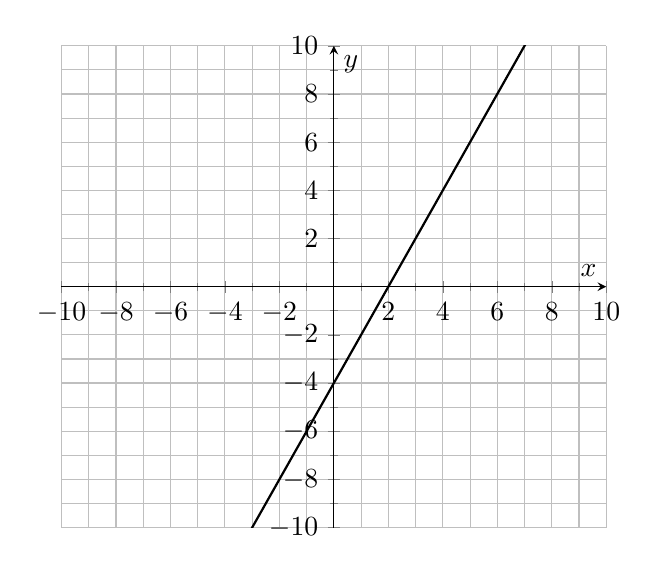
\begin{tikzpicture}
    \begin{axis}[height=7.7cm,width=8.5cm,
        axis lines=center,
        ylabel={$y$},
        xlabel={$x$},
        ymin=-10,ymax=10,
        xmin=-10,xmax=10,
        ytick={-10,-8,...,10},
        xtick={-10,-8,...,10},
        grid=both, 
        minor y tick num=1,
        minor x tick num=1,
    ]
        \addplot[thick,domain=-10:10] {2*x + -4};
        % \ifprintanswers
        %     \addplot[red,only marks,mark=*] coordinates{#3};
        % \fi
    \end{axis}
\end{tikzpicture}

\begin{randomizechoices}
    \correctchoice $2$
    \choice $\frac{1}{2}$
    \choice $4$
    \choice $\frac{1}{4}$
\end{randomizechoices}

\question
What is the speed of the car, in miles per hour (mi/h)?

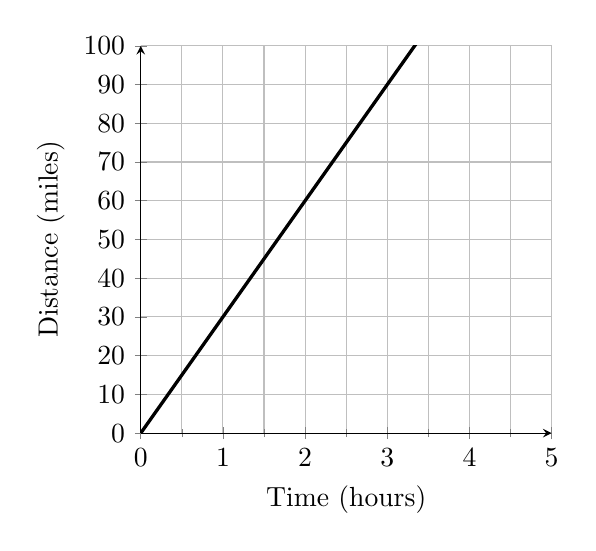
\begin{tikzpicture}
    \begin{axis}[height=6.5cm,width=6.8cm,
        axis lines=left,
        xlabel = {Time (hours)},
        ylabel = {Distance (miles)},
        ymin=0, ymax=100,
        xmin=0, xmax=5,
        ytick={0,10,...,100},
        xtick={0,1,...,5},
        minor x tick num=1,
        grid=both,
        ]
        \addplot[very thick,domain=0:5] {30*x};
    \end{axis}
\end{tikzpicture}

\begin{randomizechoices}
    \correctchoice \SI{30}{mi/h}
    \choice \SI{270}{mi/h}
    \choice \SI{45}{mi/h}
    \choice \SI{15}{mi/h}
\end{randomizechoices}

\question
Find the area of the rectangle.

\begin{center}
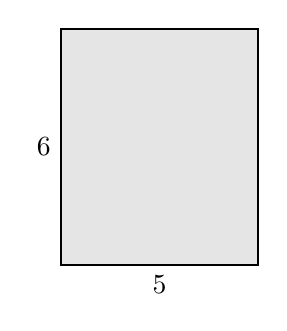
\begin{tikzpicture}[y=1mm*5,x=1mm*5]
    \draw[thick,fill=black!10] (0,0) -- (5,0) node[below,pos=0.5] {5} -- (5,6) -- (0,6) -- cycle node[left,pos=0.5] {6};
\end{tikzpicture}
\end{center}

\begin{randomizechoices}
    \correctchoice 30
    \choice 11
    \choice 0.83
    \choice 1
\end{randomizechoices}

\question
The speed graph below represents the motion of a car. How far does the car travel in\\ \underline{one and a half hours}?

\begin{tikzpicture}[y=3cm,x=5cm]
    \draw (0,0) node[below left=-1mm] {0} -- (0,1) node[rotate=90,pos=0.5,shift={(0,9mm)}] {speed (miles/hour)};
    \draw (0,0.5) -- ++(-1mm,0) node[left] {70};
    \draw (0,0) -- (1,0) node[right] {$t$} node[below=5mm,pos=0.5] {time (hours)};
    \draw (0.5,1mm) -- ++(0,-1mm) node[below] {1};
    \draw[very thick] (0,0.5) -- (1,0.5);
    \draw (0.25,1mm) -- ++(0,-1mm) node[below] {$\frac{1}{2}$};
    \draw (0.75,1mm) -- ++(0,-1mm) node[below] {$1.5$};
    \ifprintanswers
        \begin{pgfonlayer}{background}
            \fill[red!20] (0,0) rectangle (0.75,0.5);
            \draw[line width=0.4mm,{Triangle}-] (0.38,0.3) -- ++(0,0.3) node[above,shift={(9mm,0)}] {Area = 105 miles};
        \end{pgfonlayer}
    \fi
\end{tikzpicture}

\begin{randomizechoices}
    \correctchoice \SI{105}{miles}
    \choice \SI{70}{miles}
    \choice \SI{35}{miles}
    \choice \SI{90}{miles}
\end{randomizechoices}

\question
An object travels from point A to point B. Find the distance $d$ and displacement $\Delta x$ for the trip.

\begin{center}
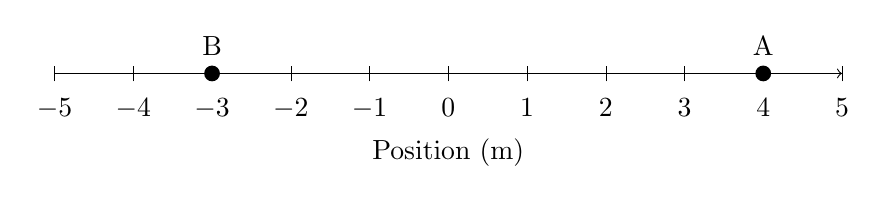
\begin{tikzpicture}[y=1cm,x=1cm]
    \foreach \x in {-5,-4,...,5} {
        \draw[ultra thin] (\x,-1mm) -- (\x,1mm) node[below=3mm] {$\x$};
    }
    \draw[->] (-5,0) -- (5,0) node[below=7mm,pos=0.5] {Position (m)};
    \fill (4,0) circle (1mm) node[above=1mm] {A};
    \fill (-3,0) circle (1mm) node[above=1mm] {B};
\end{tikzpicture}
\end{center}

\begin{randomizechoices}
    \correctchoice $d = \SI{7}{m}\ , \quad \Delta x = \SI{-7}{m}$
    \choice $d = \SI{-7}{m}\ , \quad \Delta x = \SI{-7}{m}$
    \choice $d = \SI{-7}{m}\ , \quad \Delta x = \SI{7}{m}$
    \choice $d = \SI{7}{m}\ , \quad \Delta x = \SI{7}{m}$
\end{randomizechoices}

\question
A particle moves from point A to point B in 12 seconds. Find the particle' average speed and average velocity $\bar{v}$.

\begin{center}
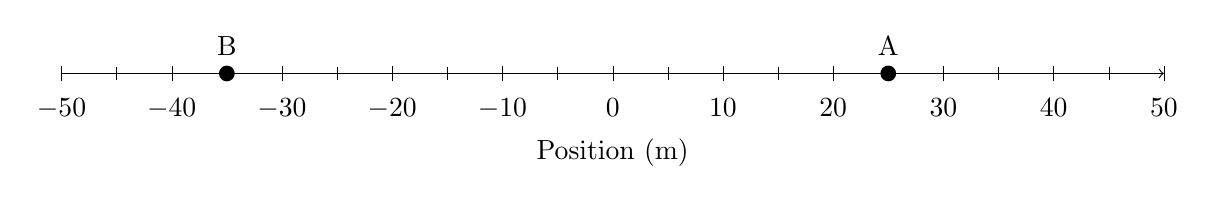
\begin{tikzpicture}[y=1.4mm,x=1.4mm]
    \foreach \x in {-50,-40,...,50} {
        \draw[ultra thin] (\x,-1mm) -- (\x,1mm) node[below=3mm] {$\x$};
    }
    \foreach \x in {-45,-35,...,45} {
        \draw[ultra thin] (\x,-0.8mm) -- (\x,0.8mm);
    }
    \draw[->] (-50,0) -- (50,0) node[below=7mm,pos=0.5] {Position (m)};
    \fill (25,0) circle (1mm) node[above=1mm] {A};
    \fill (-35,0) circle (1mm) node[above=1mm] {B};
\end{tikzpicture}
\end{center}

\begin{randomizechoices}
    \correctchoice $\text{speed} = \SI{5}{m/s}\ , \quad \bar{v} = -\SI{5}{m/s}$
    \choice $\text{speed} = -\SI{3}{m/s}\ , \quad \bar{v} = -\SI{3}{m/s}$
    \choice $\text{speed} = -\SI{3}{m/s}\ , \quad \bar{v} = \SI{3}{m/s}$
    \choice $\text{speed} = \SI{5}{m/s}\ , \quad \bar{v} = \SI{5}{m/s}$
\end{randomizechoices}

\question
The side of each grid square below represents 1 meter. A particle travels at a constant speed of 3 meters per second in the positive direction. Which of the following correctly depicts the particle's motion map?

\newcommand{\positionfigureVI}[2]{
\begin{tikzpicture}[y=5mm,x=5mm]
    \draw[black!20,step=1] (0,0) grid (24,2);
    \node[above] at (12,2) {Figure #2};
    \ifprintanswers
    \foreach \x in {0,#1,...,24}{
        \fill (\x,1) circle (0.9mm);
    }
    \fi
\end{tikzpicture}
}

\begin{center}
\positionfigureVI{1}{A}

\positionfigureVI{8}{B}

\positionfigureVI{6}{C}

{\ifprintanswers \color{red}\fi \positionfigureVI{3}{D}}
\end{center}

\begin{randomizeoneparchoices}[norandomize]
    \choice Figure A
    \choice Figure B
    \choice Figure C
    \correctchoice Figure D
\end{randomizeoneparchoices}

\question
Identify the figure that correct shows the person's position vector.

\newcommand{\positionfigureI}[4]{%
\begin{tikzpicture}[y=1cm,x=1cm]
    \foreach \x in {-5,-4,...,5} {
        \draw[ultra thin] (\x,-1mm) -- (\x,1mm) node[below=2mm] {$\x$};
    }
    \draw[->] (-5,0) -- (5,0) node[below=6mm,pos=0.5] {Position (m)} node[left=1cm,pos=0] {\bfseries Figure #4};
    \node[above] at (#1,0) {\Strichmaxerl[2]};
    \draw[very thick,->] (#2,0.7) -- (#3,0.7) node[above,pos=0.5] {$\vec{x}$};
\end{tikzpicture} 
}

\begin{center}
    \positionfigureI{-3}{-5}{-3}{A}

    \positionfigureI{-3}{5}{-3}{B}

    \positionfigureI{-3}{-3}{0}{C}

    {\ifprintanswers \color{red} \fi 
    \positionfigureI{-3}{0}{-3}{D}}
\end{center}

\begin{randomizeoneparchoices}[norandomize]
    \choice Figure A
    \choice Figure B
    \choice Figure C
    \correctchoice Figure D
\end{randomizeoneparchoices}

\question
The figure below shows 5 one-dimensional vectors. 

\begin{center}
%...PRO TIP: Use a random number generator to generate random vectors between -10 and 10
\begin{tikzpicture}[x=5mm,y=5mm]
    \draw[step=1,lightgray] (0,0) grid (10,4);
    \draw[->,line width=0.6mm,-{Triangle}] (5,4) -- ++(-3,0);
    \draw[->,line width=0.6mm,-{Triangle}] (0,3) -- ++(10,0);
    \draw[->,line width=0.6mm,-{Triangle}] (10,2) -- ++(-7,0);
    \draw[->,line width=0.6mm,-{Triangle}] (7,1) -- ++(-6,0);
    \draw[->,line width=0.6mm,-{Triangle}] (5,0) -- ++(2,0);
\end{tikzpicture}
\end{center}

Which of the following represents the vector sum of those 5 vectors?

\begin{center}
    
\end{center}





\end{questions}
\end{document}